\documentclass[11pt]{article}
\usepackage[a4paper,margin=25mm]{geometry}
\usepackage[T1]{fontenc}
\usepackage{lmodern,microtype,amsmath,amssymb,amsthm,mathtools,booktabs,tabularx,array,xcolor,enumitem,graphicx}
\usepackage[hidelinks]{hyperref}
\newcolumntype{Y}{>{\raggedright\arraybackslash}X}
\setlength{\emergencystretch}{3em}
\sloppy
\definecolor{prospectivered}{RGB}{185,0,0}
\newenvironment{prospective}{\color{prospectivered}}{}
\newtheorem{proposition}{Proposition}

\title{\textbf{Multiband Gauge Structure, Aligned Operators, and Hopping Locality}}
\author{Eugene Joseph M. Ragasa\\Department of Physics, De La Salle University, Manila, Philippines}
\date{Pre-results working manuscript}
\begin{document}
\maketitle

\begin{prospective}
\noindent\textbf{Working-color convention.} Red text identifies prospective work,
open controls, unexecuted calculations, or conditional conclusions. Extracted finite
calculations remain black and retain their historical scope.
\end{prospective}

\begin{abstract}
A composite Bloch spectrum does not identify a unique retained frame or a unique
matrix-valued hopping representation. We formulate the multiband extension of the
band-equivalence/locality program in terms of retained projectors, periodic frames,
complex unitary gauge classes, explicitly admissible alignments, and complete
matrix-valued Fourier blocks. Retained rank-two controls establish the distinction
between pointwise and global alignment and then demonstrate common-witness and
certified-separation logic under a nonidentity constrained family. Historical rank-three
calculations extracted
from Paper 1 v2 demonstrate finite-mesh
gauge consistency alongside large changes in spread and hopping tails, including one
algorithm-selected Wannier90 frame. These controls
motivate, but do not replace, a higher-rank protocol with independent verification and
separately qualified projection, frame, conversion, and truncation channels.
\end{abstract}

\section{State spaces before multiband comparison}
Let $P(\mathbf k)$ be a constant-rank spectral projector and let $F(\mathbf k):\mathbb C^r\to\mathcal H_p$ be a periodic orthonormal frame satisfying $F F^\dagger=P$. The retained matrix field is

\begin{equation}
H_F(\mathbf k)=F^\dagger(\mathbf k)H_p(\mathbf k)F(\mathbf k).
\end{equation}
A second frame $F'(\mathbf k)=F(\mathbf k)G(\mathbf k)$ gives

\begin{equation}
H_{F'}(\mathbf k)=G^\dagger(\mathbf k)H_F(\mathbf k)G(\mathbf k),
\qquad G(\mathbf k)\in U(r).
\end{equation}
The spectra and projectors are unchanged, while the represented matrices and hopping blocks generally change. A different retained rank requires a separately justified projection or embedding. Without a declared map between the spaces, an operator subtraction is undefined rather than merely large.

Spectral projection, orbital projection, disentanglement, downfolding, frame selection, and hopping truncation are distinct operations. In particular, an exact spectral projector commutes with the parent, whereas an orbital-semantic projector generally does not. The latter may require an energy-dependent Feshbach--Löwdin operator or a separately qualified unitary decoupling.

\section{Pointwise and global unitary alignment}
Given reference and candidate frames of equal rank, define the cross-overlap

\begin{equation}
M(\mathbf k)=F_{\mathrm{cand}}^\dagger(\mathbf k)F_{\mathrm{ref}}(\mathbf k)
=L(\mathbf k)\Sigma(\mathbf k)V^\dagger(\mathbf k).
\end{equation}
When the declared pointwise alignment family is the complete unitary group, the polar factor

\begin{equation}
U(\mathbf k)=L(\mathbf k)V^\dagger(\mathbf k)
\end{equation}
minimizes the pointwise Frobenius frame residual. A one-global-unitary comparison instead uses

\begin{equation}
B=\sum_{\mathbf k}F_{\mathrm{cand}}^\dagger(\mathbf k)
F_{\mathrm{ref}}(\mathbf k)=L_B\Sigma_BV_B^\dagger,
\qquad U_{\mathrm{glob}}=L_BV_B^\dagger.
\end{equation}
These are different admissible alignment families, not two numerical approximations to the same problem. A rank-deficient cross-overlap or aggregate leaves an undetermined unitary action in null spaces. Equality at the declared singular-value cutoff is therefore deficient and must fail closed unless a separately reviewed completion rule is part of the protocol.

For momentum-dependent alignment, matrices are aligned before Fourier transformation:

\begin{equation}
\widetilde H(\mathbf R)
=\frac{1}{N_k}\sum_{\mathbf k}e^{-i\mathbf k\cdot\mathbf R}
U^\dagger(\mathbf k)H(\mathbf k)U(\mathbf k).
\end{equation}
This mixes hopping ranges and requires periodicity and reciprocal-boundary sewing. Wilson-loop and closure phases remain sewing diagnostics; they are not topological claims without an independently qualified continuum construction.

\subsection{Extracted rank-two alignment control}\label{sec:rank-two-alignment}
A retained four-state synthetic parent supplies an isolated lowest-two-state group. A
known smooth periodic real rotation preserves the retained projector within
$3.24\times10^{-16}$ while producing maximum frame and represented-operator defects
$1.506$ and $0.997$ in the attacked frame. Pointwise Procrustes alignment recovers the
known inverse attack within $6.77\times10^{-16}$ and reduces the operator defect to
$9.83\times10^{-16}$. In contrast, the best one-global-unitary channel leaves maximum
frame and operator defects $1.131$ and $0.744$.

The attack also lengthens the matrix-hopping tail without changing any band energy. At
range eight, its omitted block norm and withheld maximum spectral error are
$5.65\times10^{-5}$ and $7.04\times10^{-5}$, compared with approximately
$1.6\times10^{-14}$ and $1.2\times10^{-14}$ after transport or pointwise recovery.
These values establish a finite controlled alignment/locality mechanism, not a general
optimizer or continuum decay law.

\begin{figure}[htbp]
\centering
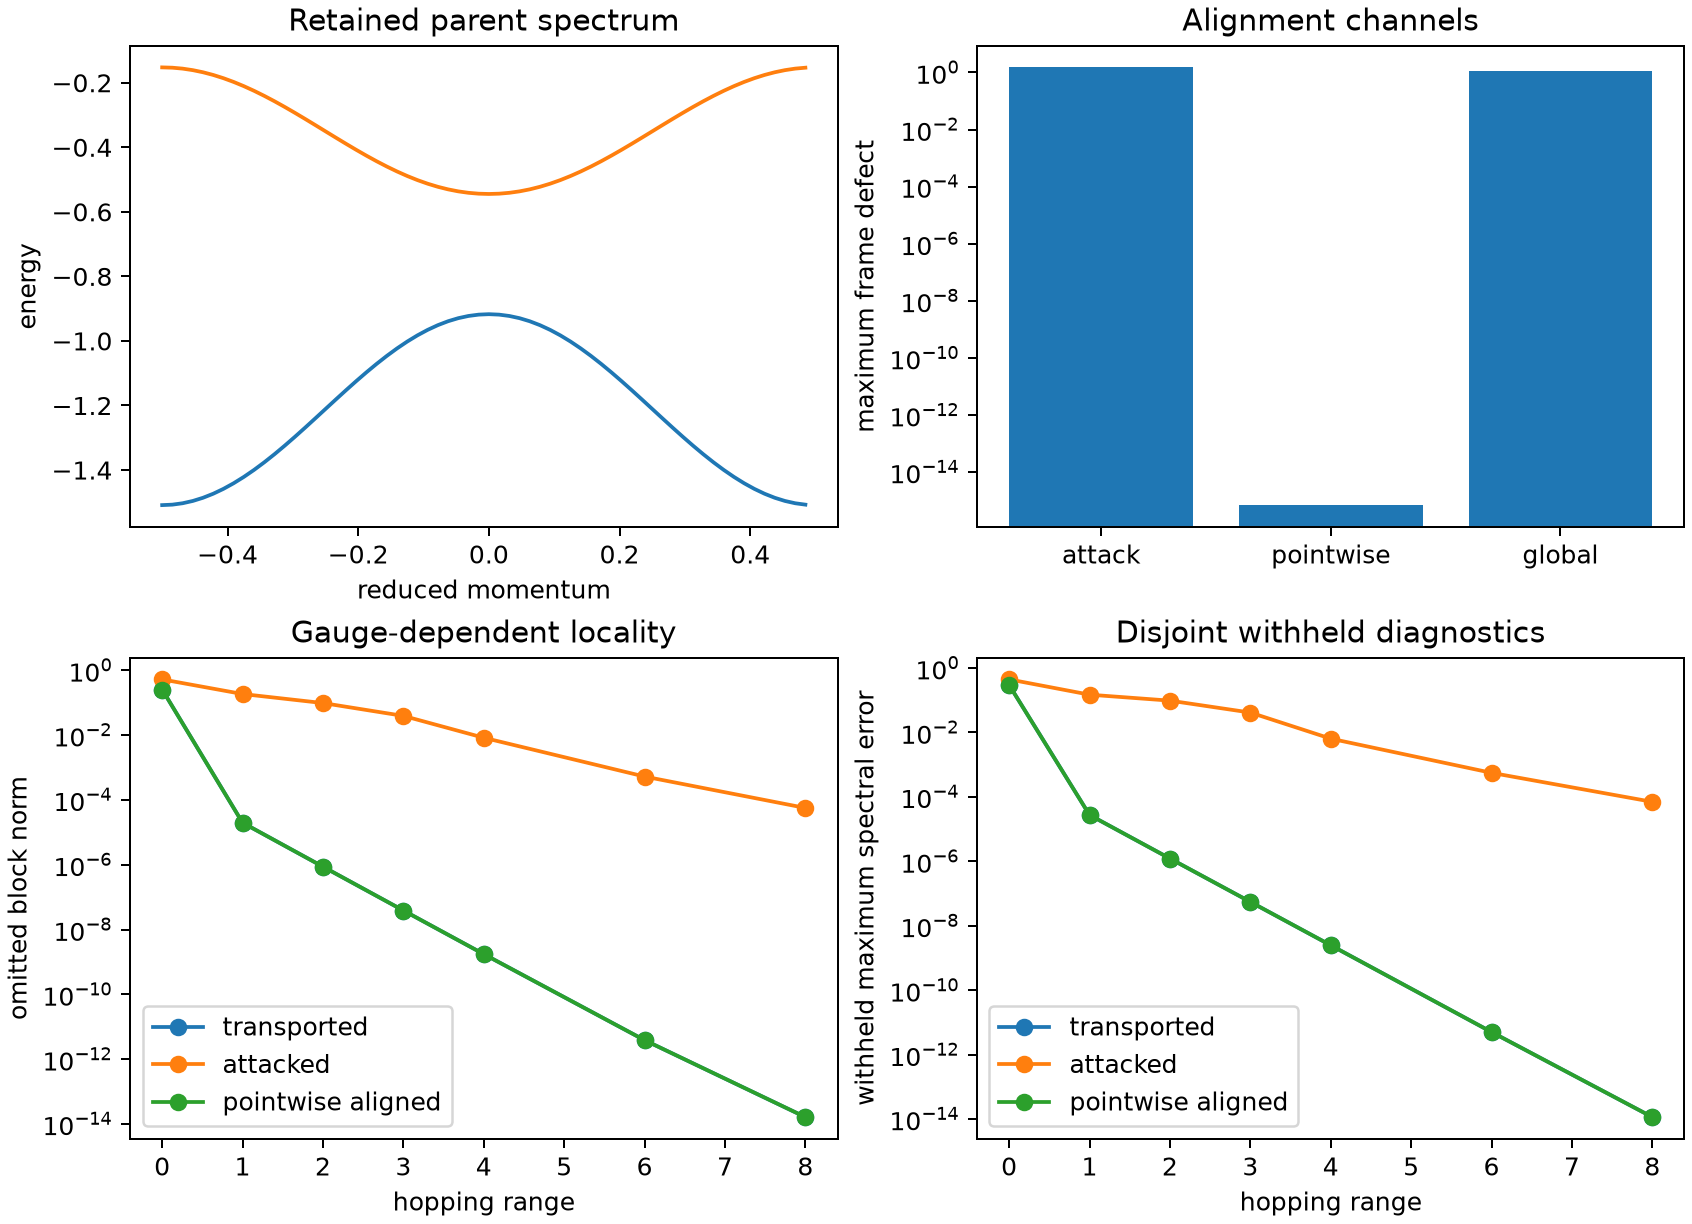
\includegraphics[width=\textwidth]{../../../../../calculations/ICMSEP2026/conference/paper_1/multiband-alignment/multiband-alignment-summary.png}
\caption{Extracted M2 rank-two control. Pointwise recovery and one-global alignment are
different admissible families; the known gauge attack preserves the retained spectrum
while changing finite-range compressibility.}
\label{fig:m2-alignment}
\end{figure}

\section{Admissible sets and bounded decisions}\label{sec:bounded-decisions}
Let $X$ be a declared model-parameter domain with metric $d$, and let
$L_E(\boldsymbol\theta)$ and $L_{H,\mathrm{orb}}(\boldsymbol\theta)$ be frozen spectral
and aligned-operator losses. The latter includes minimization only over the declared
admissible alignment family. For fixed thresholds, define
\begin{align}
 \mathcal A_E&=\{\boldsymbol\theta\in X:L_E(\boldsymbol\theta)\le\tau_E\},\\
 \mathcal A_H&=\{\boldsymbol\theta\in X:L_{H,\mathrm{orb}}(\boldsymbol\theta)\le\tau_H\},\\
 \delta^*&=\inf_{\substack{\boldsymbol\theta_E\in\mathcal A_E\\
                           \boldsymbol\theta_H\in\mathcal A_H}}
 d(\boldsymbol\theta_E,\boldsymbol\theta_H).
 \label{eq:set-separation}
\end{align}

\begin{proposition}[Witnesses and certified separation]
\label{prop:witness-separation}
For nonempty $\mathcal A_E$ and $\mathcal A_H$, a common witness in their intersection
proves $\delta^*=0$. Every feasible pair supplies an upper bound on $\delta^*$. A
certified bound $0<\underline\delta\le\delta^*$ proves that the sets are disjoint.
Failure of a search or local optimizer to find a common witness proves none of these
statements. If both sets are compact and disjoint, their distance is attained and
strictly positive; without compactness, disjoint nonempty sets can have zero distance.
\end{proposition}

\begin{proof}
A common witness supplies a feasible equal pair of distance zero. Any other feasible
pair bounds the defining infimum from above, while a positive certified lower bound
excludes an intersection. If both sets are compact, their Cartesian product is compact
and the continuous distance function attains its minimum. A zero attained minimum would
identify a common point, so disjointness makes that minimum positive. A failed search
supplies neither a witness nor a lower bound.
\end{proof}

If either set is empty, the corresponding single-criterion feasibility test fails; this
manuscript does not replace that outcome by a finite set-to-set distance. The proposition
is general decision bookkeeping, not a claim that an arbitrary nonconvex separation has
been computed.

\subsection{Controlled rank-two common-witness precursor}
The retained M3 calculation from Paper 1 v2 starts from a transported rank-two reference
$H(k)$ and uses the two-parameter candidate below. Here $E_{\mathrm{ref}}>0$ is an
arbitrary reference-energy normalization, not a band gap:
\begin{equation}
 H_{s,\lambda}(k)=\overline E(k)I+sE_{\mathrm{ref}}I
 +\lambda\left[H(k)-\overline E(k)I\right],
 \qquad (s,\lambda)\in[-0.25,0.25]\times[0.4,1.2].
\end{equation}
Its operator comparison minimizes over the prospectively frozen family of nine constant
real rotations with angles from $-1.2$ to $1.2$ radians. It excludes the
momentum-dependent pointwise alignment that recovers the constructed frame attack.

With spectral threshold $\tau_E=0.03$ and operator threshold $\tau_H=0.33$, the original
candidate $(s,\lambda)=(0,1)$ passes both requirements using the nonidentity constant
alignment $\phi=0.3$. Its training losses are
\begin{equation}
 L_E(0,1)=7.59\times10^{-16},
 \qquad
 L_H(0,1;\phi=0.3)=0.3286318914.
\end{equation}
This retained point is the common witness in the left panel of
Fig.~\ref{fig:m3-admissible-sets}; compatibility does not follow merely from visual
boundary overlap.

Keeping $\tau_E=0.03$ but tightening the operator threshold to $\tau_H=0.31$ moves the
closest spectral and operator boundary points to splitting scales
$0.9354687052$ and $0.8360013041$. The analytic quadratic certificate gives
\begin{equation}
 \delta^*=0.0994674010>0.05,
\end{equation}
where $0.05$ is the frozen separation resolution. This positive certified distance,
not failure of a search, gives the separated disposition in the right panel.

\begin{figure}[htbp]
\centering
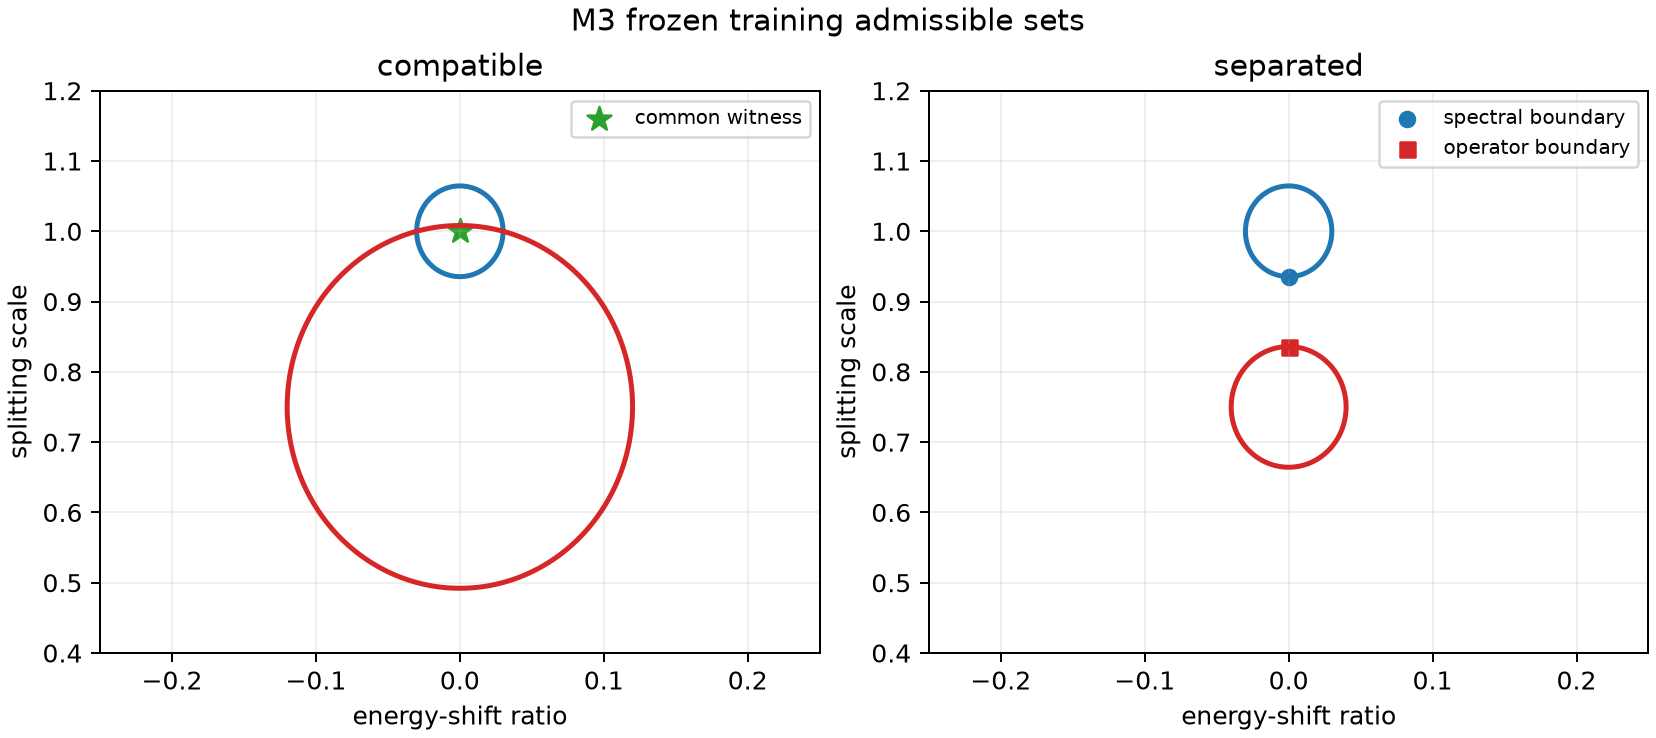
\includegraphics[width=\textwidth]{../../../../../calculations/ICMSEP2026/conference/paper_1/constrained-admissible-sets/constrained-admissible-sets-summary.png}
\caption{Retained M3 rank-two admissible sets extracted from Paper 1 v2. At the compatible
threshold, the nonidentity $0.3$-radian constant alignment admits the explicit common
witness $(0,1)$ (left). Tightening only the operator threshold produces certified
separation within the same frozen nine-angle family (right). The panels do not compare
an unrestricted pointwise alignment with no alignment.}
\label{fig:m3-admissible-sets}
\end{figure}

This precursor directly exercises a constrained multiband alignment family, but only a
finite one. It does not establish a continuous or momentum-dependent optimizer, a
higher-rank result, or transferable physical thresholds. Its role is to demonstrate the
common-witness and certified-separation decisions before the higher-rank alignment
families below introduce additional feasibility and conditioning questions.

\section{Extracted rank-three two-dimensional evidence}\label{sec:rank-three}
A retained two-dimensional calculation compared a smooth projected frame with a periodic rough internal gauge for the lowest three bands. The two frames agreed spectrally within $1.22\times10^{-15}E_{\mathrm{ref}}$ and in unordered discrete Wilson-loop eigenphases within $2.22\times10^{-15}$. The finite-mesh winding diagnostic was zero in both frames. Nevertheless, their common finite-supercell spread estimators were $24.90a^2$ and $67.70a^2$, while the omitted hopping norms beyond squared-radius shell 18 were $1.38\times10^{-2}E_{\mathrm{ref}}$ and $5.25\times10^{-1}E_{\mathrm{ref}}$.

These values establish a finite rank-three gauge/locality control. They do not certify a continuum Chern invariant, a global localization optimum, or a material Hamiltonian.

\begin{figure}[htbp]
\centering
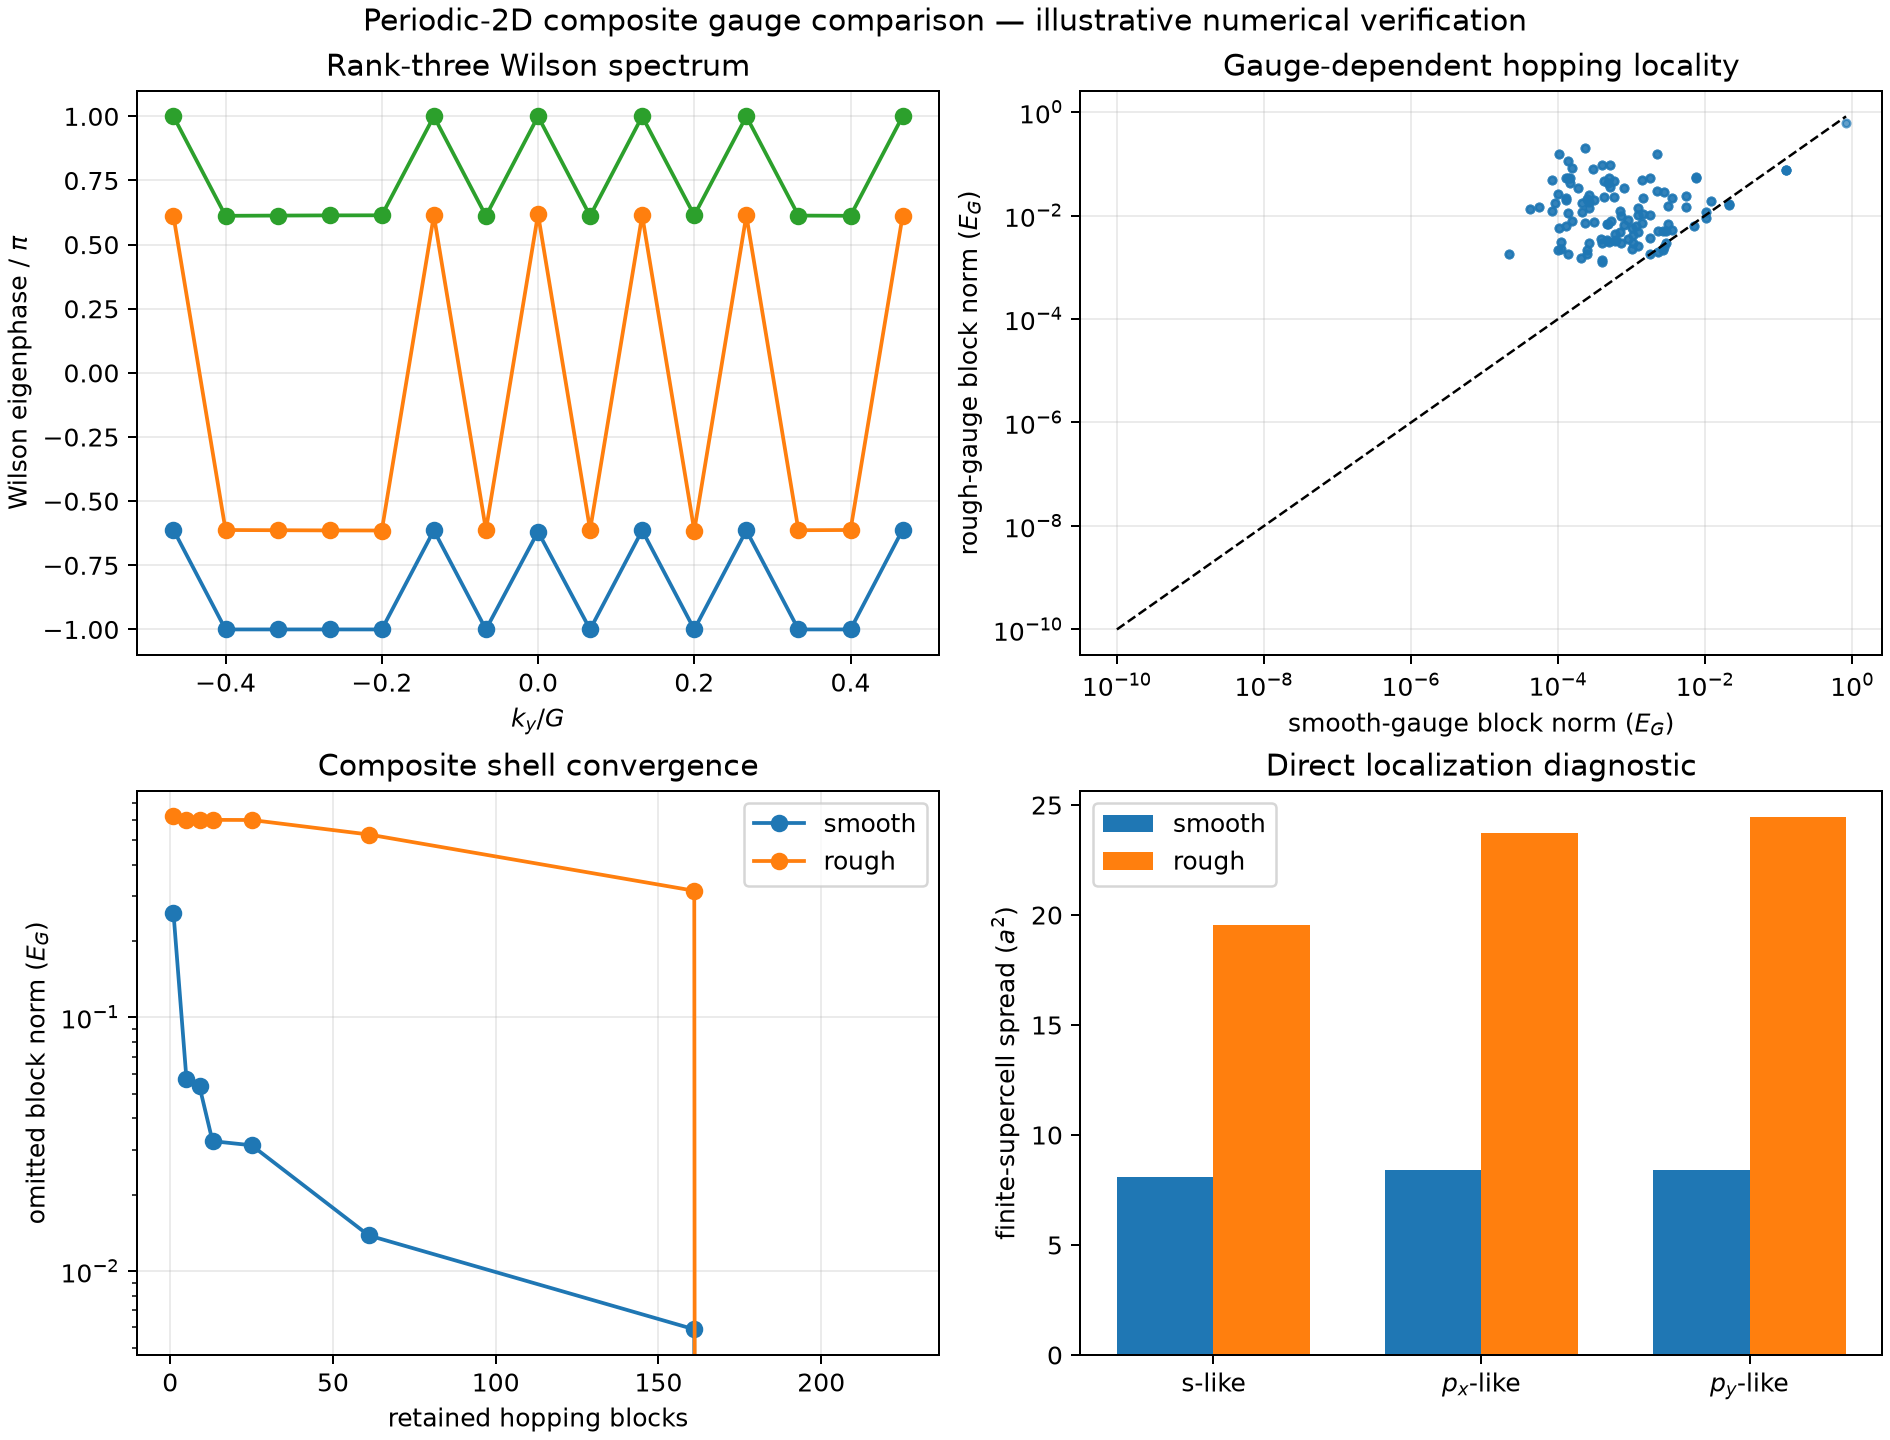
\includegraphics[width=\textwidth]{../../../../../calculations/research-monograph/periodic-2d/composite-summary.png}
\caption{Extracted rank-three smooth/rough-gauge comparison. Gauge-invariant finite-mesh
subspace and spectral diagnostics coexist with different spread estimators and hopping
tails.}
\label{fig:rank-three-gauge}
\end{figure}

\section{Extracted algorithm-selected Wannier90 bridge}\label{sec:wannier-bridge}
A separate synthetic two-dimensional calculation used Wannier90 3.1.0 on a $15\times15\times1$ mesh with three trial projections and no disentanglement. The direct projected and Wannier90-selected frames had maximum projector discrepancy $2.65\times10^{-10}$. Pointwise identification reduced their represented-operator discrepancy to $3.57\times10^{-10}E_{\mathrm{ref}}$. A bounded family allowing integer orbital translations in $[-1,1]^2$ followed by one constant orbital unitary instead left an operator discrepancy of $1.490E_{\mathrm{ref}}$.

Under one common finite-supercell estimator, the Wannier90 and direct-frame spreads were $6.1359a^2$ and $24.5163a^2$. At squared radius 50, their omitted hopping norms were $2.72\times10^{-4}E_{\mathrm{ref}}$ and $5.90\times10^{-3}E_{\mathrm{ref}}$. A retained six-case mesh, cutoff, and embedding study was nonmonotone and reached different localization basins. The evidence therefore supports one finite algorithm-selected comparison, not mesh-independent localization or global MLWF optimality.

\begin{figure}[htbp]
\centering
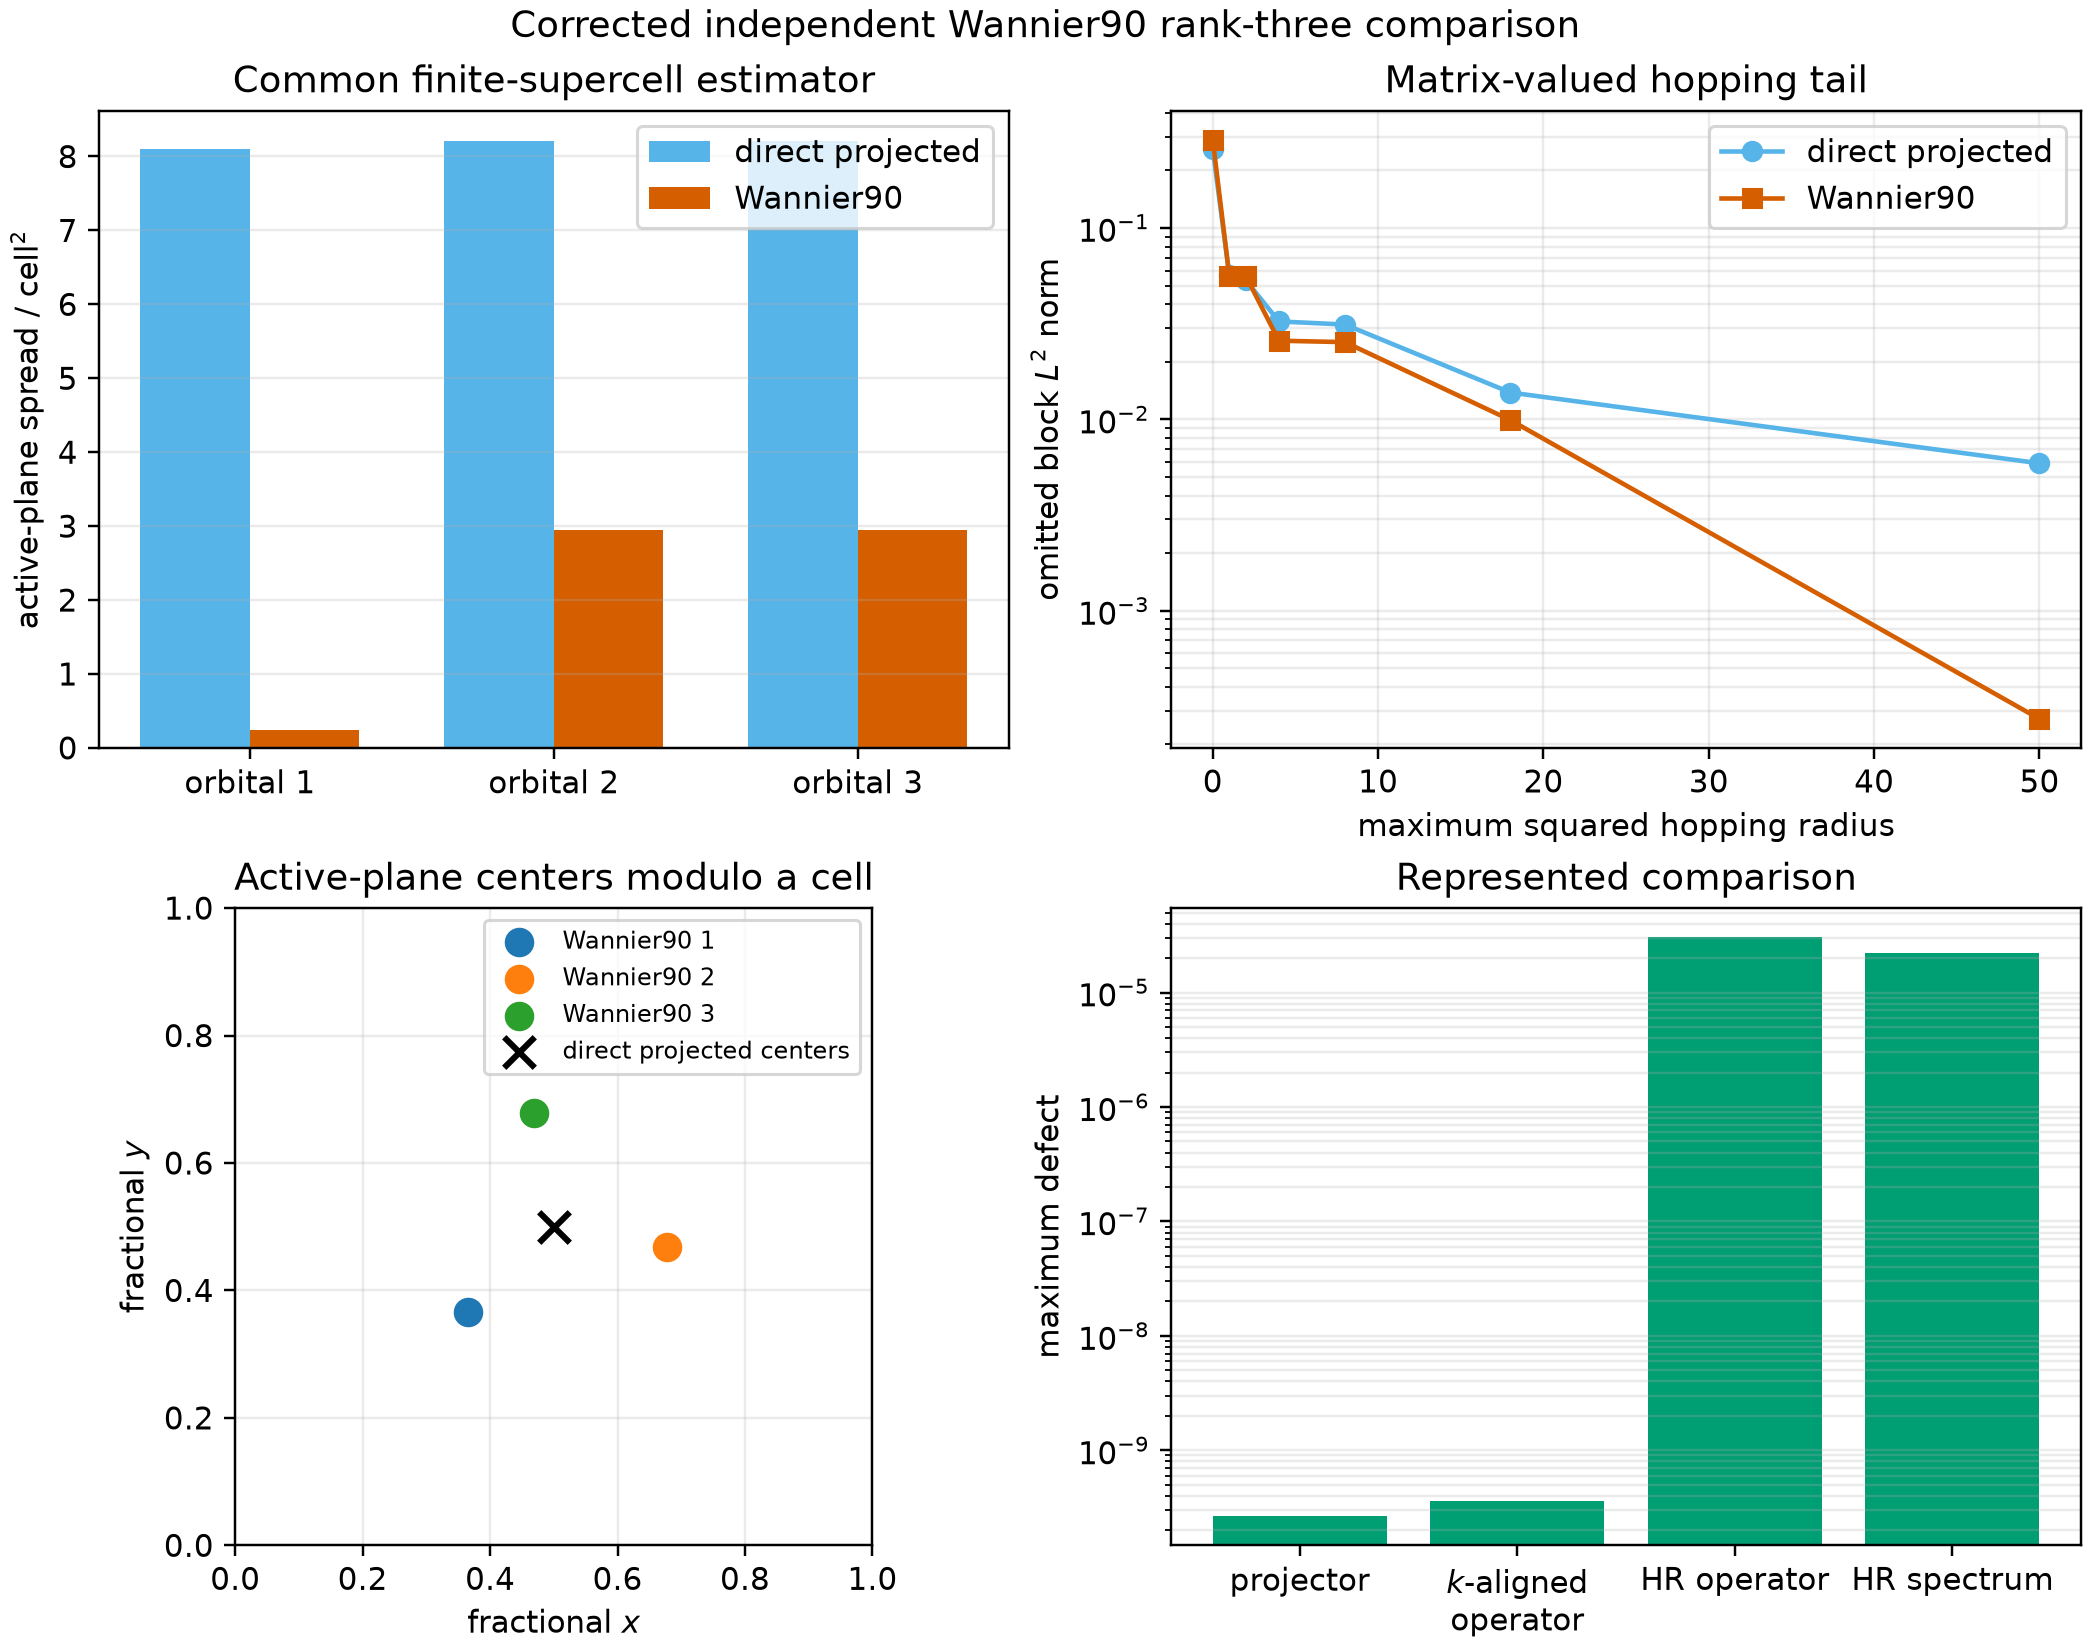
\includegraphics[width=\textwidth]{../../../../../calculations/research-monograph/periodic-2d/wannier90-balanced-summary.png}
\caption{Extracted finite rank-three Wannier90 bridge. Native and common-estimator
spreads are not interchangeable. Pointwise represented alignment, restricted global
alignment, and finite-shell hopping tails remain separate diagnostics.}
\label{fig:wannier90-bridge}
\end{figure}

\begin{prospective}
\section{Prospective multiband protocol}
Paper 3 will require a separately selected retained rank, parent family, real $SO(r)$ or
complex $U(r)$ gauge class, global-periodic-frame algorithm, rank thresholds, sewing
traversal, tensor meshes, support inventory, truncation targets, serializers, and an
independent verifier. Rank-two formulas and Paper 2 numerical controls will not be
inherited without a reviewed specialization.

The future evidence ledger will keep parent discretization, projection or
disentanglement, frame construction, covariant equivalence, restricted alignment,
Fourier conversion, interpolation, deliberate truncation, and total Hamiltonian and
spectral consequences separate. No combined diagnostic score is planned.

\section{Results boundary}
No new Paper 3 numerical result, experiment identity, protocol freeze, retained run, or
evidence package exists. New conclusions may be added only after a higher-rank protocol
is frozen and independently verified. The extracted rank-three controls above retain
their original finite-mesh and synthetic scope.
\end{prospective}

\clearpage
\appendix
\section{Extracted evidence boundary}\label{app:evidence-boundary}
The numerical values reproduced in Sections~\ref{sec:rank-two-alignment},
\ref{sec:bounded-decisions}, \ref{sec:rank-three}, and~\ref{sec:wannier-bridge}
originate from the preserved
\texttt{conference-paper-1v2/manuscript.tex} and its cited retained calculations. This
appendix records their permitted role in Paper 3.

\begin{center}\small
\begin{tabularx}{\textwidth}{YYY}
\toprule
\textbf{Extracted component} & \textbf{Supported statement} & \textbf{Not supported} \\
\midrule
M3 constrained rank-two admissible sets & One frozen finite alignment family has an explicit nonidentity-aligned common witness and, at a tighter operator threshold, a certified positive separation & Continuous or momentum-dependent alignment, higher-rank validity, material validity, or transferable thresholds \\
M2 rank-two alignment control & A known pointwise inverse attack is recoverable while one global unitary leaves a finite residual, and the attack changes finite-range compressibility & General alignment optimizer, continuum decay law, or material validity \\
Rank-three smooth/rough frames & Finite-mesh equality of spectra and Wilson-phase multisets can coexist with different spread estimators and hopping tails & Continuum topology, material validity, or global localization optimum \\
Synthetic Wannier90 bridge & One algorithm-selected rank-three frame can be identified pointwise with the direct retained subspace while differing under a restricted global family & Mesh-independent MLWF convergence, global basin optimality, or first-principles validation \\
Procrustes construction & Pointwise and one-global unitary alignments solve different declared least-squares problems when their overlap factors are qualified & Permission to complete a rank-deficient map or enlarge the admissible family after observing results \\
\bottomrule
\end{tabularx}
\end{center}

A post-hoc exact reanalysis of the sealed M3 training quadratics places the compatibility
transition at $\tau_H=0.3192641695$ for the fixed $\tau_E=0.03$ and the declared
nine-angle family. It is sensitivity characterization, not a prospectively frozen
prediction or physical threshold calibration.

\begin{figure}[htbp]
\centering
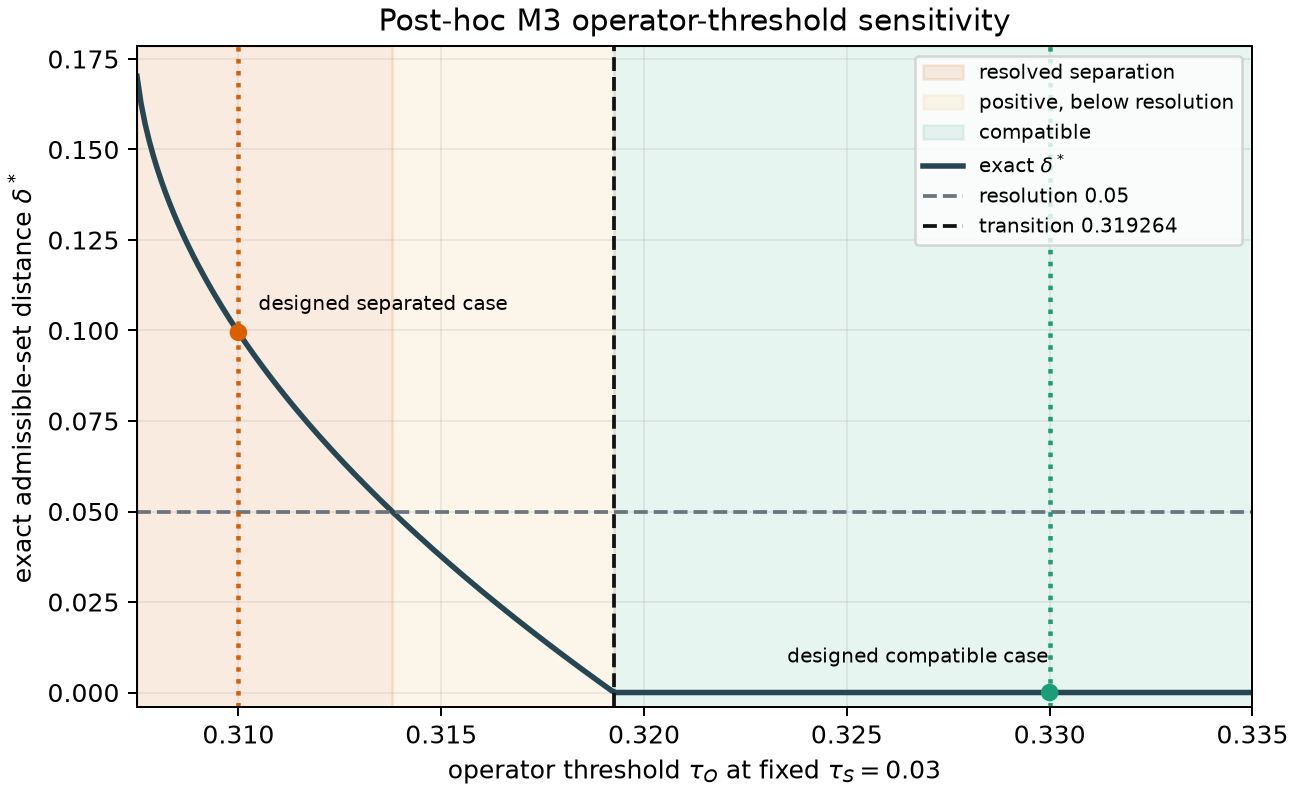
\includegraphics[width=0.84\textwidth]{../../../../../calculations/ICMSEP2026/conference/paper_1/constrained-admissible-sets-threshold-sensitivity/operator-threshold-sensitivity.png}
\caption{Post-hoc M3 operator-threshold sensitivity. The sealed compatible and separated
thresholds lie on opposite sides of the exact finite-family transition.}
\label{fig:m3-threshold-sensitivity}
\end{figure}

\begin{figure}[htbp]
\centering
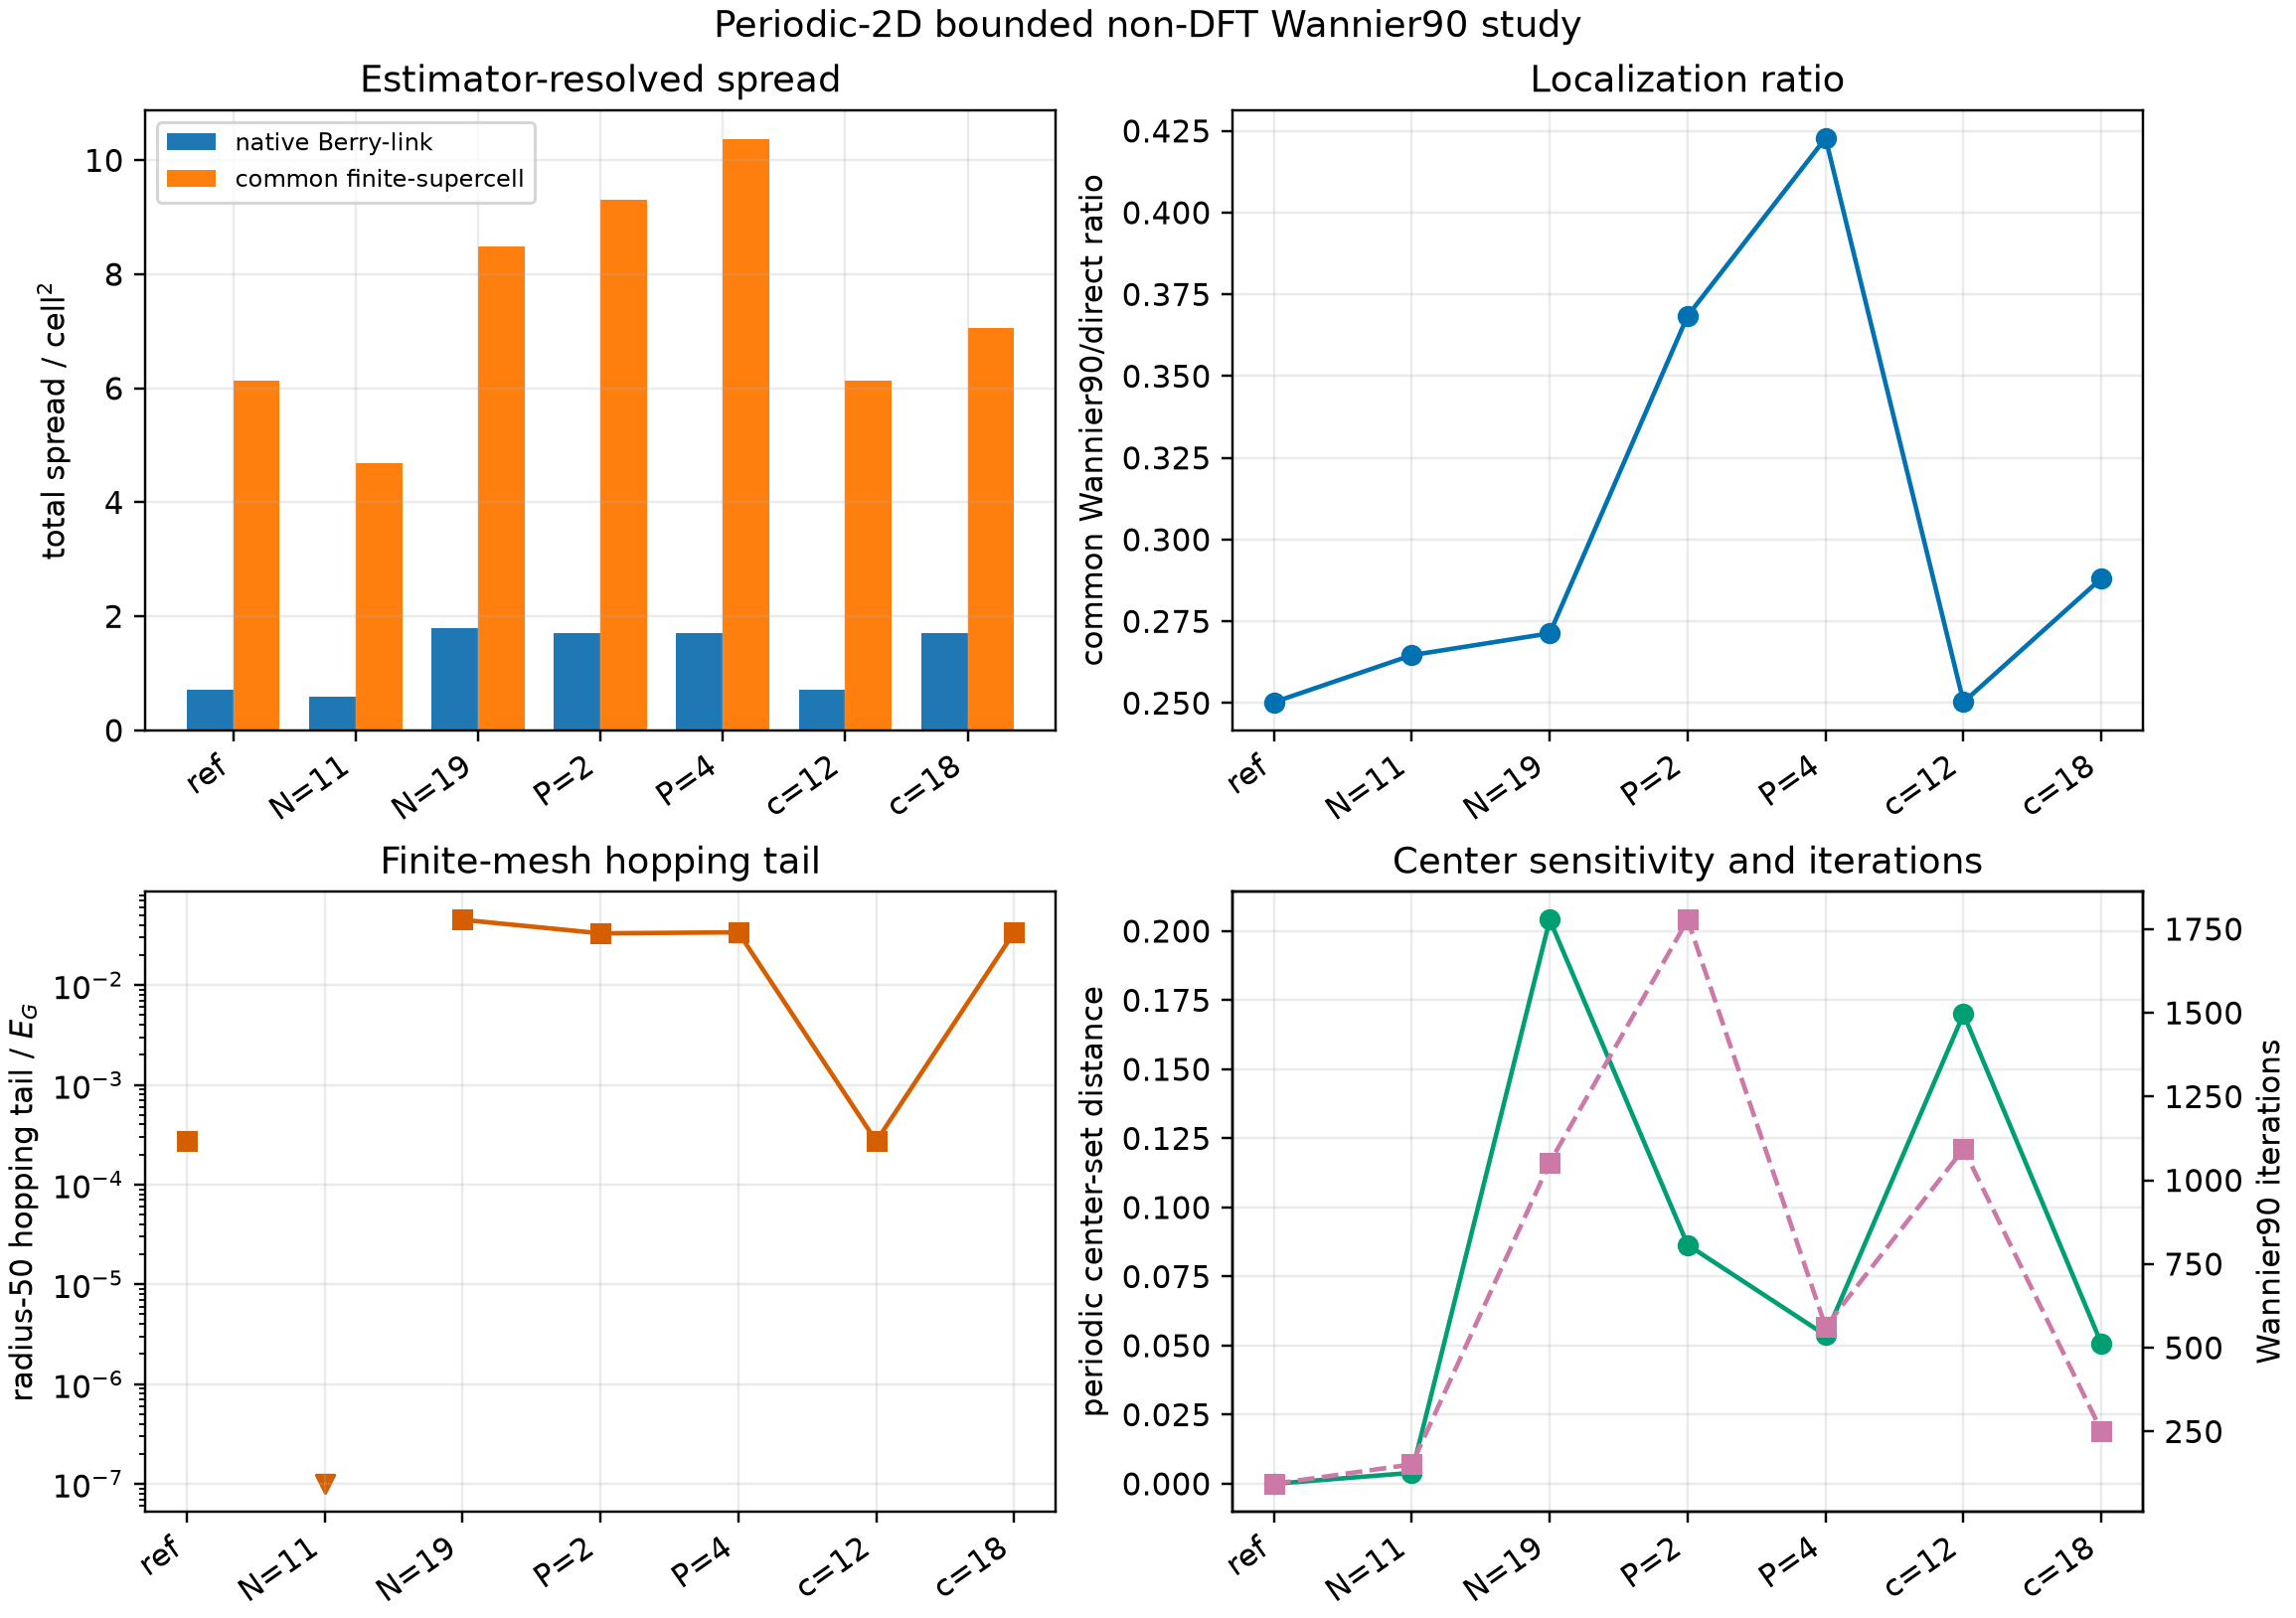
\includegraphics[width=\textwidth]{../../../../../calculations/research-monograph/periodic-2d/wannier90-study-summary.png}
\caption{Extracted Wannier90 sensitivity record. Mesh, plane-wave cutoff, and inactive
embedding variations reach nonmonotone spreads, tails, centers, and optimizer iteration
counts. The zero radius-50 tail for $N=11$ is finite-support bookkeeping, not an
infinite-range conclusion.}
\label{fig:wannier90-sensitivity}
\end{figure}

No Paper 1 threshold, finite-angle inventory, mesh, tolerance, source identity, or evidence identity is transferred into a future Paper 3 experiment. A new higher-rank calculation requires its own protocol, schemas, verifier, convergence result, and evidence qualification.

\end{document}
